\documentclass[10pt,twocolumn]{article}
\usepackage[margin=0.75in]{geometry}
\usepackage[T1]{fontenc}
\usepackage[utf8]{inputenc}
\usepackage{amsmath,amssymb}
\usepackage{booktabs}
\usepackage{graphicx}
\usepackage{caption}
\usepackage[hidelinks]{hyperref}
\usepackage{natbib}
\bibliographystyle{plainnat}
\captionsetup{font=small,labelfont=bf}
\setlength{\parskip}{2pt}

\title{\vspace{-1.5em}\Large A simulation environment for market making under
adverse selection, and how learned and closed-form controls behave in it}
\author{Hamidou Diallo}
\date{}

\begin{document}
\maketitle

\begin{abstract}
\small
We extend the \texttt{mbt\_gym} simulator so that a market maker's executions carry information about where the
price is going next, and we measure how far the Avellaneda--Stoikov and Cartea--Jaimungal controls degrade as
that effect is strengthened. Five reinforcement learning algorithms are trained in the same environment on a
feature set that does not contain the latent factor. Two results follow. The closed forms lose most or all of
their value once the effect is strong, while the learned agents keep roughly two fifths of theirs. More
importantly, the learned agents hold terminal inventory almost fixed across an eightfold change in the strength
of the effect, whereas the derived closed forms let it grow by a factor of three to ten. Terminal inventory is
what the criterion prices, so this is the binding constraint of the problem rather than a secondary statistic.
\end{abstract}

\section{The control problem}

A market maker quotes a bid at $S_t - \delta^-_t$ and an ask at $S_t + \delta^+_t$ around a reference price
$S_t$, and is filled when an incoming market order matches one of the quotes. Write $q_t$ for the inventory
carried, $X_t$ for cash, and $N^{+}_t, N^{-}_t$ for the counting processes of filled sell and buy limit orders.
Inventory and cash follow
\begin{align}
dq_t &= dN^-_t - dN^+_t, \\
dX_t &= (S_t + \delta^+_t)\,dN^+_t - (S_t - \delta^-_t)\,dN^-_t .
\end{align}

The objective is the criterion of \citet{cartea2015book}:
\begin{equation}
J \;=\; \underbrace{X_T + q_T S_T}_{\text{terminal wealth}}
\;-\; \varphi \int_0^T q_t^2\,dt \;-\; \alpha\, q_T^2 ,
\label{eq:criterion}
\end{equation}
with $T$ the horizon, $\varphi \ge 0$ the price of carrying inventory through time, and $\alpha \ge 0$ the cost
of liquidating whatever position is left at $T$. The last term is a liquidation cost under linear price impact:
unwinding $q$ units degrades the average execution price by $\alpha q$ and therefore costs $\alpha q^2$.

Two properties of the resulting optimal control matter throughout. Under the assumptions it is derived from, the
optimal depths are
\begin{equation}
\delta^{\pm,*}(t,q) \;=\; \tfrac{1}{\kappa} + h_q(t) - h_{q \mp 1}(t),
\label{eq:cj}
\end{equation}
where $\kappa$ is the decay rate of the fill probability and $h$ solves a linear system indexed by inventory.
The control therefore depends on $(t, q)$ and on four constants, and on nothing else. In particular it carries no
state through which an exogenous signal could enter. This is not a defect of the formula; it is its scope, and it
is the reason a degradation study is informative.

\section{The simulated market}

The base simulator is \texttt{mbt\_gym} \citep{jerome2022mbtgym}. Table~\ref{tab:params} lists every parameter
used. Prices are continuous, one fill moves inventory by one unit, and the horizon is divided into $200$ steps.

\begin{table}[t]
\small\centering
\caption{Parameters. The first block is the market, the second the criterion, the third the three mechanisms
described in Section~\ref{sec:mechanisms}. Only $\gamma$ is varied.}
\label{tab:params}
\begin{tabular}{llr}
\toprule
symbol & meaning & value \\
\midrule
$T$, $n$ & horizon, steps & $1.0$, $200$ \\
$S_0$ & initial price & $100$ \\
$\sigma$ & price volatility & $2.0$ \\
$\lambda$ & order arrival rate per side & $140$ \\
$\kappa$ & fill probability decay & $1.5$ \\
$Q$ & inventory bound & $20$ \\
\midrule
$\varphi$ & inventory carried & $0.01$ \\
$\alpha$ & inventory left at $T$ & $1.0$ \\
\midrule
$\gamma$ & signal strength & \textbf{varied} \\
$p$ & probability of being served & $0.95$ \\
$\zeta$ & own trade price impact & $0.1$ \\
\bottomrule
\end{tabular}
\end{table}

\subsection{Three mechanisms}
\label{sec:mechanisms}

\paragraph{Informational adverse selection.}
This is the object of the study. A mean reverting factor $\alpha_t$, unrelated to the constant $\alpha$ of
Eq.~\eqref{eq:criterion}, drives both the price drift and the direction of order flow:
\begin{align}
dS_t &= \alpha_t\,dt + \sigma\,dW_t, \\
\lambda^{\text{sell}}(\alpha_t) &= \lambda e^{-\gamma \alpha_t}, \quad
\lambda^{\text{buy}}(\alpha_t) = \lambda e^{+\gamma \alpha_t}.
\end{align}
When the factor is positive the price drifts up and buy orders become more frequent. Those orders lift the maker's
ask, so it sells just before the rise. The correlation between fills and later price moves is not imposed: it
follows from the two channels sharing one factor. Setting $\gamma = 0$ recovers independent Poisson arrivals
exactly, which makes the classical environment a limiting case of this one.

\paragraph{Queue position and own trade impact.}
Two further mechanisms are present but held fixed. With probability $1-p$ a matching order does not reach the
maker's quote, which stands for not being first in the queue. And each fill moves the reference price by $\zeta$
in the direction of the aggressor, so that the maker is pushed against the position it has just taken. Both are
included for realism rather than as objects of study; the second is an optimal execution effect and is not what
this report is about. Measured against a fixed reference policy, the queue mechanism costs about $5\%$ of profit
at $p = 0.95$ and the impact mechanism about $6\%$ at $\zeta = 0.1$. A third mechanism available in the code, in
which the price trading through a resting quote forces a fill \citep{lalor2024adverse}, is left switched off: at
the depths quoted here such an event is close to a five sigma move and the mechanism is numerically inert.

\section{Agents}

\subsection{Closed forms, and their refitted counterparts}

Two analytic controls are used. Avellaneda--Stoikov \citep{avellaneda2008} maximises the exponential utility of
terminal wealth and reads a risk aversion, a volatility and a fill decay. Cartea--Jaimungal
\citep{cartea2015book} maximises Eq.~\eqref{eq:criterion} directly and reads $\kappa$, $\lambda$, $\varphi$ and
$\alpha$. Deployed unchanged in the enriched market, each is simply misspecified, and what it loses measures the
cost of that misspecification rather than the value of anything that might replace it.

Each therefore also appears in a refitted form: the same functional shape, with its own internal constants chosen
by grid search on simulated returns, refitted separately at every signal strength. No parameter is added, and the
objective stays pinned to the environment's reward so every arm is scored identically. This arm should be read as
an upper reference rather than as a competitor. It runs its search inside the true environment, so it knows both
the functional form and the answer, which a deployed strategy would not. The search is scored on three fitting
seeds and reported on four disjoint evaluation seeds, because an argmax over a noisy objective buys part of its
own improvement.

\subsection{Learned agents}

Five algorithms are used, chosen to span the families the two recent surveys organise around
\citep{bai2024review, ghasemi2025survey} rather than to collect recent methods. Table~\ref{tab:agents} lists them.
Reinforcement learning has been applied to market making since \citet{chan2001}, whose state variables are
inventory, order imbalance, spread and recent price changes; the feature set below was arrived at independently
and is very nearly the same.

\begin{table}[t]
\small\centering
\caption{The five algorithms and why each is present. All share a two layer network of width $64$ with ReLU
activations and the discount fixed to one, since the criterion is an undiscounted finite horizon sum. Everything
else is left at library defaults.}
\label{tab:agents}
\begin{tabular}{lp{4.6cm}}
\toprule
algorithm & role \\
\midrule
PPO \citep{schulman2017ppo} & on policy with a trust region; the usual reference in this literature \\
A2C \citep{mnih2016a3c} & the same without the trust region, which isolates what clipping buys \\
SAC \citep{haarnoja2018sac} & off policy, maximum entropy; sample efficient \\
TD3 \citep{fujimoto2018td3} & off policy, deterministic policy, twin critics \\
Recurrent PPO & PPO with an LSTM; the factor is latent, so the sufficient statistic is a function of history \\
\bottomrule
\end{tabular}
\end{table}

\paragraph{What the agent sees.}
The latent factor is never given to a learned agent. Its features are inventory, time remaining, the imbalance and
the total count of recent order arrivals, the imbalance of its own recent fills, and the return over a recent
window. All are quantities a market maker observes. Two windows are used, five steps for the count based features
and twenty for the return, because the first is limited by arrival noise and the second by how fast the factor
itself moves; the two optima were measured, not assumed.

\section{Method}

\paragraph{Nesting.}
Every mechanism has a setting at which the enriched environment must reproduce the classical one trajectory by
trajectory, not merely in distribution. This is asserted by test, and it is what makes the analytic control a
limiting case rather than an out of distribution baseline whose gap would be uninterpretable.

\paragraph{Replication.}
A learned arm is trained on three seeds and each trained policy is evaluated on four further seeds, disjoint from
the training ones and shared across all arms, with $1500$ trajectories per seed. The spread reported for a learned
arm is taken across training seeds, since two runs of one algorithm differ and that is the variability that
matters when comparing algorithms. For an analytic arm the spread is taken across evaluation seeds. Every arm sees
the same evaluation seeds, so comparisons between arms are paired.

\paragraph{How degradation is measured.}
An arm is first measured in the environment with the mechanism switched off, which gives it a reference value.
The mechanism is then strengthened and the arm is measured again, unchanged. We report the share of its own
reference value that it retains. An arm that scored $60$ and now scores $24$ has kept $40\%$ of what it had. This
is a within arm comparison, so it does not reward an arm for having been strong to begin with.

\paragraph{Quantities reported.}
Alongside the criterion of Eq.~\eqref{eq:criterion} we report four quantities that do not depend on how the
criterion prices risk: terminal wealth, its standard deviation across trajectories, the mean absolute inventory
held at the horizon, and the number of orders filled per episode. A change visible only in the criterion is a
statement about the scoring; a change visible in these four is a statement about behaviour.

\section{Results}

\subsection{Value kept as the effect strengthens}

Figure~\ref{fig:degradation} shows, for each arm, the share of its own reference value retained as the signal
strength rises from zero to $0.8$. The two analytic controls fall below zero: at the strongest setting
Cartea--Jaimungal ends at $-31\%$ of its reference value and Avellaneda--Stoikov at $-79\%$, meaning both destroy
value rather than merely earning less. The refitted controls and the three learned agents stay in a narrow band
between $13\%$ and $40\%$.

\begin{figure}[t]
\centering
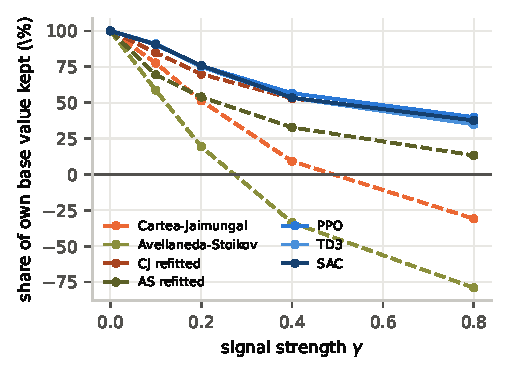
\includegraphics[width=\columnwidth]{figures/degradation.pdf}
\caption{Share of its own reference value that each arm retains. Solid lines are learned agents, dashed lines are
analytic controls. The horizontal line at zero separates arms that still earn from arms that lose. Reading the
right hand edge: the learned agents and the refitted Cartea--Jaimungal keep between a third and two fifths, while
the two derived controls are below zero.}
\label{fig:degradation}
\end{figure}

Table~\ref{tab:main} gives the full picture at the strongest setting. The criterion column separates the arms
into those that still work and those that do not. The four columns to its right are independent of how the
criterion prices risk.

\begin{table}[t]
\small\centering
\caption{All arms at signal strength $0.8$. Criterion is Eq.~\eqref{eq:criterion}; wealth is its first term; the
last column is orders filled per episode, with the share of the same arm's own count at zero signal in
parentheses.}
\label{tab:main}
\begin{tabular}{lrrrrr}
\toprule
arm & crit. & wealth & vol. & $|q_T|$ & orders \\
\midrule
Cartea--J. & $-18.4$ & $25.1$ & $29.2$ & $4.39$ & $74\ (76\%)$ \\
Avell.--S. & $-38.9$ & $26.6$ & $13.5$ & $6.74$ & $60\ (65\%)$ \\
CJ refit. & $22.1$ & $30.1$ & $13.2$ & $1.79$ & $41\ (43\%)$ \\
AS refit. & $6.5$ & $22.5$ & $7.0$ & $3.35$ & $31\ (34\%)$ \\
\midrule
PPO & $22.1$ & $23.4$ & $7.6$ & $\mathbf{0.81}$ & $25\ (32\%)$ \\
TD3 & $19.5$ & $20.3$ & $6.8$ & $\mathbf{0.59}$ & $31\ (38\%)$ \\
SAC & $21.0$ & $22.4$ & $7.7$ & $\mathbf{0.85}$ & $35\ (39\%)$ \\
\bottomrule
\end{tabular}
\end{table}

\subsection{Terminal inventory}

The criterion prices whatever position is left at the horizon, so holding that position near zero is the binding
constraint of the problem rather than a secondary statistic. Figure~\ref{fig:inventory} tracks it.

\begin{figure}[t]
\centering
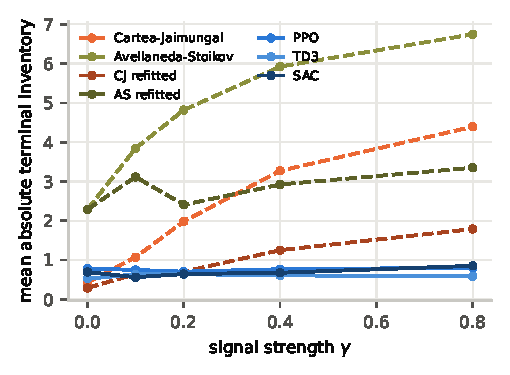
\includegraphics[width=\columnwidth]{figures/inventory.pdf}
\caption{Mean absolute inventory held at the horizon. The three learned agents are the flat lines near the bottom.
Over an eightfold increase in signal strength their terminal inventory changes by at most a quarter, while the
derived Cartea--Jaimungal control multiplies its own by ten.}
\label{fig:inventory}
\end{figure}

The learned agents hold terminal inventory between $0.53$ and $0.86$ units at every signal strength. Over the same
range the derived Cartea--Jaimungal control goes from $0.43$ to $4.39$, a factor of ten, and the refitted one from
$0.29$ to $1.79$, a factor of six. Avellaneda--Stoikov never reads the reward function at all, so its policy is
identical at every setting and its inventory rises to $6.74$ purely because the market changed underneath it.

This is the clearest separation in the study, and it is not close. At the strongest setting the learned agents end
with two to eight times less inventory than any analytic arm, and they do so while giving up less wealth per unit
of its standard deviation.

\subsection{Activity}

A control can always reduce what adverse selection costs it by quoting wider and trading less. Whether the arms
do that is visible in the last column of Table~\ref{tab:main} and in Figure~\ref{fig:orders}.

\begin{figure}[t]
\centering
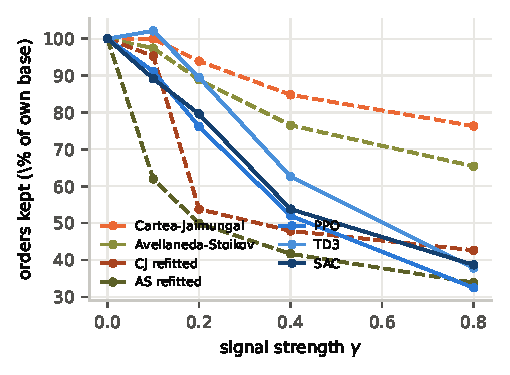
\includegraphics[width=\columnwidth]{figures/orders.pdf}
\caption{Orders filled per episode, as a share of the same arm's count at zero signal. Every arm that still earns
value cuts activity to between a third and two fifths. The arm that keeps trading most is also the one that ends
worst.}
\label{fig:orders}
\end{figure}

All arms that retain value converge to a similar level of activity, between $32\%$ and $43\%$ of their own base
count. The learned agents are inside that band, not above it: they are not more active than the refitted control.
What the figure does show is that activity is not by itself a virtue. The derived Cartea--Jaimungal control keeps
$76\%$ of its orders, the highest of any arm, and it is the arm that loses the most value. It keeps quoting into
flow that has turned against it, which is exactly the failure the mechanism was built to produce.

The right reading is therefore that reducing activity is necessary but not sufficient, and that the arms are
separated by what they do with the orders they keep. Per order filled, markout at a five step horizon is $-0.10$
to $-0.12$ for the learned agents against $-0.17$ for the refitted control and $-0.21$ for the derived one, so the
flow the learned agents retain is roughly half as toxic.

\subsection{An asymmetry in the protocol}

The only arm that matches the learned agents on the criterion is the refitted Cartea--Jaimungal control, and the
comparison is not symmetric. That arm searches over its own constants inside the true environment, once per
setting, so it is given both the functional form and the answer. The learned agents received no tuning: library
default hyperparameters, one network size, no architecture or learning rate search, with only the discount fixed
because the criterion requires it. The protocol is tilted toward the analytic side, and the learned agents still
match it on the criterion while ending with less inventory and less toxic flow.

\section{Limits}

The measurements above hold inside one simulated market, and four limits bound what they say.

\paragraph{The quoted spread is wide relative to the volatility.}
The controls quote about $67$ basis points around a price whose one step move is $14$ basis points. A liquid
futures contract has a spread two orders of magnitude tighter relative to its volatility. The consequence is that
the price essentially never trades through a resting quote, so the mechanical channel of
\citet{lalor2024adverse} is inert and only the informational channel is exercised. Reaching the other regime is a
joint constraint on the fill decay, the volatility and the step size, not a setting to switch.

\paragraph{The signal is generous.}
At one standard deviation of the factor the two arrival intensities differ by a factor of six. Order flow
predictability in traded data is far weaker. The strongest setting used here should be read as an extreme case
rather than a central one.

\paragraph{Volatility is constant.}
There are no calm and turbulent regimes, so the ability to widen when the market turns is not tested. A stochastic
variance process is implemented and verified to reproduce the constant case exactly when its volatility of
volatility is zero, but activating it was measured to change the reference policy's outcome by under two
percent, so it is left off. Making regimes matter would require coupling the variance to the arrival intensity,
which is a modelling choice rather than a parameter.

\paragraph{Budget.}
The learned agents are compared at a fixed number of environment steps. Their criterion is still rising with
training at that point, so any ordering read at one budget is a statement about that budget. Longer runs move the
learned agents up relative to the refitted control; the point at which they cross it is a property of this
configuration and of the compute spent, not a quantity worth reporting on its own.

\section{Conclusion}

Strengthening the informational component of adverse selection degrades every control in the study, which is
expected: neither analytic control carries a state through which the factor could enter, and this is visible in
their formulas. What the measurements add is how differently the arms degrade.

The derived controls do not merely earn less, they stop working, ending below zero once the effect is strong. The
learned agents keep about two fifths of their own reference value, which is close to what a control refitted
inside the true environment keeps.

The separation that is not close is inventory. The learned agents hold terminal inventory almost fixed across an
eightfold change in the strength of the effect, while the analytic controls let it grow by a factor of three to
ten. Since the criterion prices exactly that quantity, and since the agents reach it without being given the
latent factor and without any hyperparameter tuning, this is the result we would carry forward.

Two things this does not establish. It does not show that a learned agent would hold up in a market calibrated to
traded data, since the environment here is not; and it does not separate what the agents learn about the factor
from what they learn about inventory control, since both improve together. The natural next step is a policy with
oracle access to the factor, which would bound how much of the remaining gap is attributable to prediction.

\section*{Reproducibility}

The environment, the agents, the training scripts and the evaluation notebooks are in the project repository.
Trained policies are regenerated by the training scripts; every number in this report comes from an executed
notebook.

\begin{thebibliography}{99}
\small
\bibitem[Avellaneda and Stoikov(2008)]{avellaneda2008}
M.~Avellaneda and S.~Stoikov.
High frequency trading in a limit order book.
\emph{Quantitative Finance}, 8(3):217--224, 2008.

\bibitem[Bai et al.(2024)]{bai2024review}
Y.~Bai, Y.~Gao, R.~Wan, S.~Zhang, and R.~Song.
A review of reinforcement learning in financial applications.
\emph{arXiv:2411.12746}, 2024.

\bibitem[Cartea et al.(2015)]{cartea2015book}
{\'A}.~Cartea, S.~Jaimungal, and J.~Penalva.
\emph{Algorithmic and High-Frequency Trading}.
Cambridge University Press, 2015.

\bibitem[Cartea and Jaimungal(2016)]{cartea2016flow}
{\'A}.~Cartea and S.~Jaimungal.
Incorporating order-flow into optimal execution.
\emph{Mathematics and Financial Economics}, 10(3):339--364, 2016.

\bibitem[Chan and Shelton(2001)]{chan2001}
N.~T. Chan and C.~Shelton.
An electronic market-maker.
MIT AI Lab Technical Report, 2001.

\bibitem[Fujimoto et al.(2018)]{fujimoto2018td3}
S.~Fujimoto, H.~van Hoof, and D.~Meger.
Addressing function approximation error in actor-critic methods.
\emph{ICML}, 2018.

\bibitem[Ghasemi et al.(2025)]{ghasemi2025survey}
M.~Ghasemi, A.~H. Moosavi, and D.~Ebrahimi.
Comprehensive survey of reinforcement learning: from algorithms to practical challenges.
\emph{arXiv:2411.18892}, 2025.

\bibitem[Haarnoja et al.(2018)]{haarnoja2018sac}
T.~Haarnoja, A.~Zhou, P.~Abbeel, and S.~Levine.
Soft actor-critic: off-policy maximum entropy deep reinforcement learning with a stochastic actor.
\emph{ICML}, 2018.

\bibitem[Jerome et al.(2022)]{jerome2022mbtgym}
J.~Jerome, L.~S{\'a}nchez-Betancourt, R.~Savani, and M.~Herdegen.
mbt-gym: reinforcement learning for model-based limit order book trading.
\emph{arXiv:2209.07823}, 2022.

\bibitem[Lalor and Swishchuk(2024)]{lalor2024adverse}
L.~Lalor and A.~Swishchuk.
Market simulation under adverse selection.
\emph{arXiv:2409.12721}, 2024.

\bibitem[Mnih et al.(2016)]{mnih2016a3c}
V.~Mnih et al.
Asynchronous methods for deep reinforcement learning.
\emph{ICML}, 2016.

\bibitem[Schulman et al.(2017)]{schulman2017ppo}
J.~Schulman, F.~Wolski, P.~Dhariwal, A.~Radford, and O.~Klimov.
Proximal policy optimization algorithms.
\emph{arXiv:1707.06347}, 2017.

\bibitem[Spooner et al.(2018)]{spooner2018}
T.~Spooner, J.~Fearnley, R.~Savani, and A.~Koukorinis.
Market making via reinforcement learning.
\emph{AAMAS}, 2018.
\end{thebibliography}

\end{document}
